Im Folgenden wird ein sehr typisches Phänomen untersucht, das bei jeder Anwendung von TF auftritt. Der Verlauf der 
Performanz-Kurven für Trainings- und Validierungsdaten zeigt stets einen deutlichen Einbruch an dem Punkt, an dem das TF 
implementiert wird. Dieses Verhalten ist in Abbildung \ref{fig:convmaxpooltrain} insbesondere bei Epoche 20 deutlich erkennbar.

\begin{figure}[htpb]
    \centering
    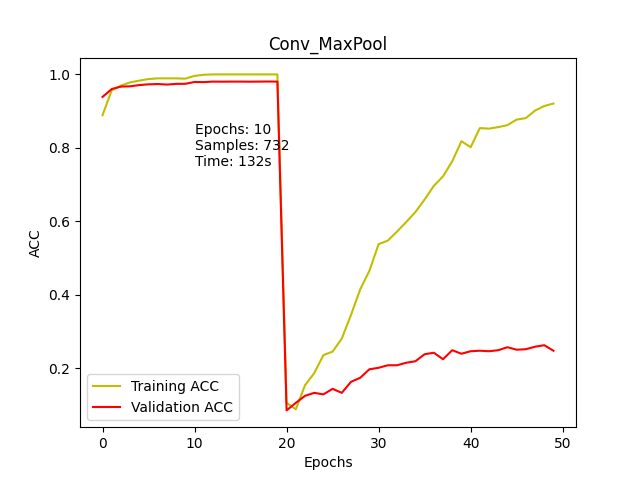
\includegraphics[height=5cm]{../../Plots/ba_plots/convmaxpool/convmaxpooltrain.png}
    \caption{\label{fig:convmaxpooltrain} 
    \small{Abgebildet ist der Test CMP:TF2/732/10. Der Fokus liegt hierbei auf Epoche 20, da zu diesem Zeitpunkt das TF 
    angewendet wurde. Infolge dessen ist ein deutlicher Einbruch der Performanz zu beobachten.}}
\end{figure}

Dieser Leistungseinbruch tritt konsistent nach der Anwendung von TF auf. Dies ist darauf zurückzuführen, dass das Netzwerk 
bislang ausschließlich auf dem Source-Datensatz trainiert wurde und somit keine Kenntnis der Target-Daten besitzt. Das Modell verfügt demnach 
nur über das Wissen aus der Source-Domäne und kann dieses initial nur auf die neue Domäne übertragen. Betrach-tet man jedoch das Testergebnis, 
das ausschließlich auf dem Target-Datensatz basiert, so ergibt sich das in Abbildung \ref{fig:convmaxpooltest} dargestellte Bild.

\begin{figure}[htpb]
    \centering
    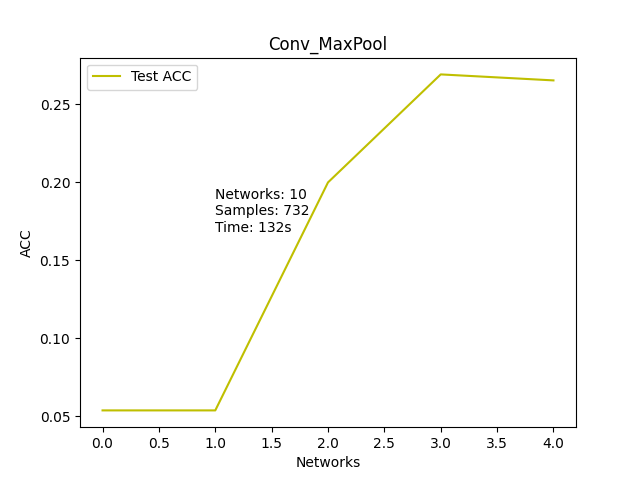
\includegraphics[height=5cm]{../../Plots/ba_plots/convmaxpool/convmaxpooltest.png}
    \caption{\label{fig:convmaxpooltest} 
    \small{Diese Abbildung zeigt den Test CMP:TF2/732/10. Dieser basiert auf Target-Daten, die dem Netzwerk während des 
    Trainings nicht zugänglich waren. Nach Abschluss des Trainings jedes Layers erfolgt eine Evaluation anhand der Testdaten. Dementsprechend 
    ist der Punkt, an dem TF durchgeführt wird, bei zwei Netzwerken erkennbar. Zu diesem Zeitpunkt verbessert sich die 
    Performanz deutlich.}}
\end{figure}

Der Wechsel erfolgt hierbei beim zweiten Netzwerk. Es ist deutlich erkennbar, dass sich die Performanz nach Anwendung des 
TFs verbessert. Dies liegt darin begründet, dass das Netzwerk ab diesem Zeitpunkt auf Trainingsdaten trainiert wird, die mit dem Testdatensatz 
übereinstimmen, da dieser ausschließlich Daten aus dem Target-Datensatz enthält.
